\section{Resultat} % (fold)
\label{sec:resultat}
    \subsection{Algoritm} % (fold)
    \label{sub:algoritm}

    % subsection algoritm (end)
    \subsection{Optisk kommunikation} % (fold)
    \label{sub:optisk_kommunikation}

        Kommunikationen mellan det upplysta rummet och solpanelen på taket kan upprättas med hjälp av två mikrokontroller, en för sändning av data och en för mottagande.\bigskip

        Den lösning som detta projekt presenterar består mikrokonrollerkortet av Arduino Uno revision 3 (för fullständig specifikation se bilaga \ref{sub:arduino_spec}).\cite{ardu} Till sändaren kopplas en lysdiod till det gränssnitt som skickar data via den seriella standarden, vilket då omvandlar från RS-232 standardens höga- och låga läge, till ljus på och ljus av. Till mottagaren kopplas en fotoresistor, en resistor som ändrar motståndet när den träffas av ljus, vilket gör att när den kopplas in till det seriella gränssnittet skapar resistorn spänningsförändringar som registreras som högt eller lågt värde av standarden. \bigskip

        För att möjliggöra överföringen används den i förhållandevis låga överföringshastigheten om 300 baud, vilket gör att komponenterna (fotoresistorn och lysdioden), hinner ändra sina värden under den tid de förväntas göra det på, då dessa komponenter inte är särskilt utformade för denna uppgift och innehåller vissa fördröjningar vid skifte av tillstånd. \bigskip

        Den data som avses skickas i denna kommunikation består av ett 16 bitars värde, det vill säga två byte. Med en överföringshastighet om 300 baud ger det en teoretisk möjlighet att skicka $\frac{300 \,\textit{baud}}{8 \, bit \cdot 2} = 18,75 \, \text{värden per sekund}$. Den faktiska hastigheten blir något lägre då extra bitar skickas enligt RS-232 protokollet, men överföringshastigheten är inte att anses som ett hinder i denna implementation.

        \begin{figure}[h]
        \centering
            \begin{subfigure}[hbt]{0.35\textwidth}
                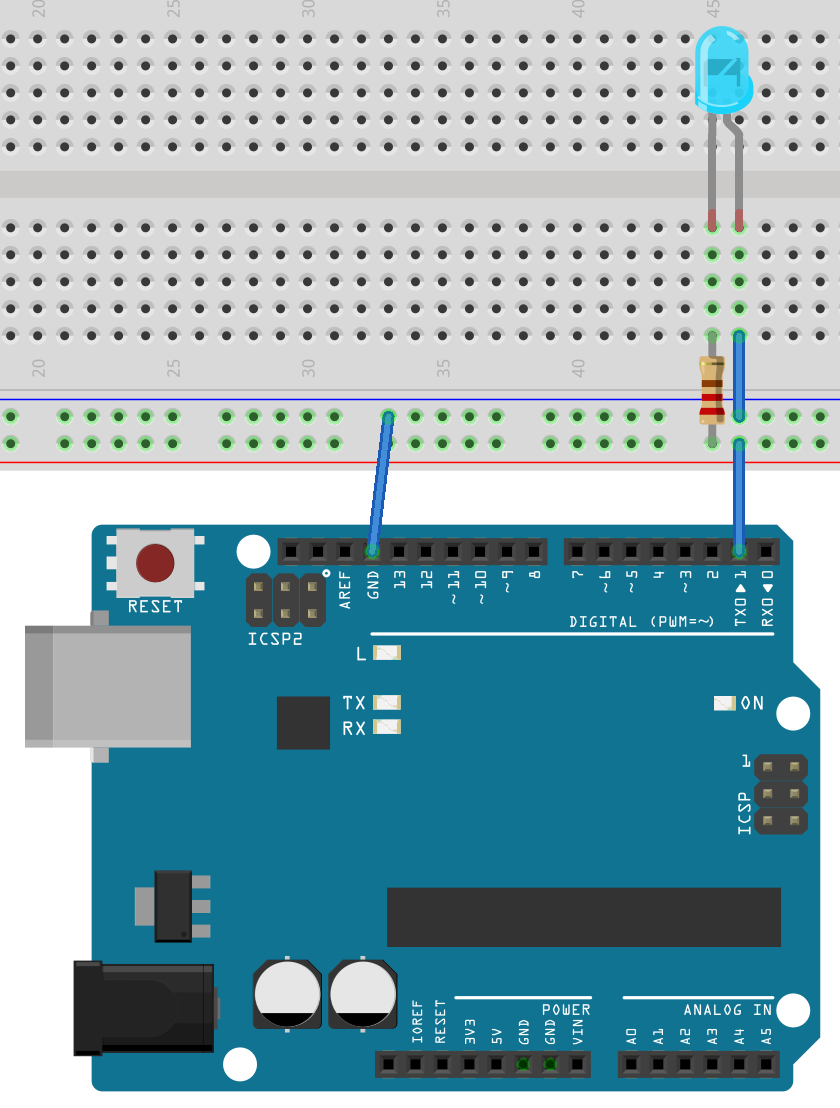
\includegraphics[width=\textwidth]{res/img/led}    
            \end{subfigure}
            \begin{subfigure}[hbt]{0.35\textwidth}
                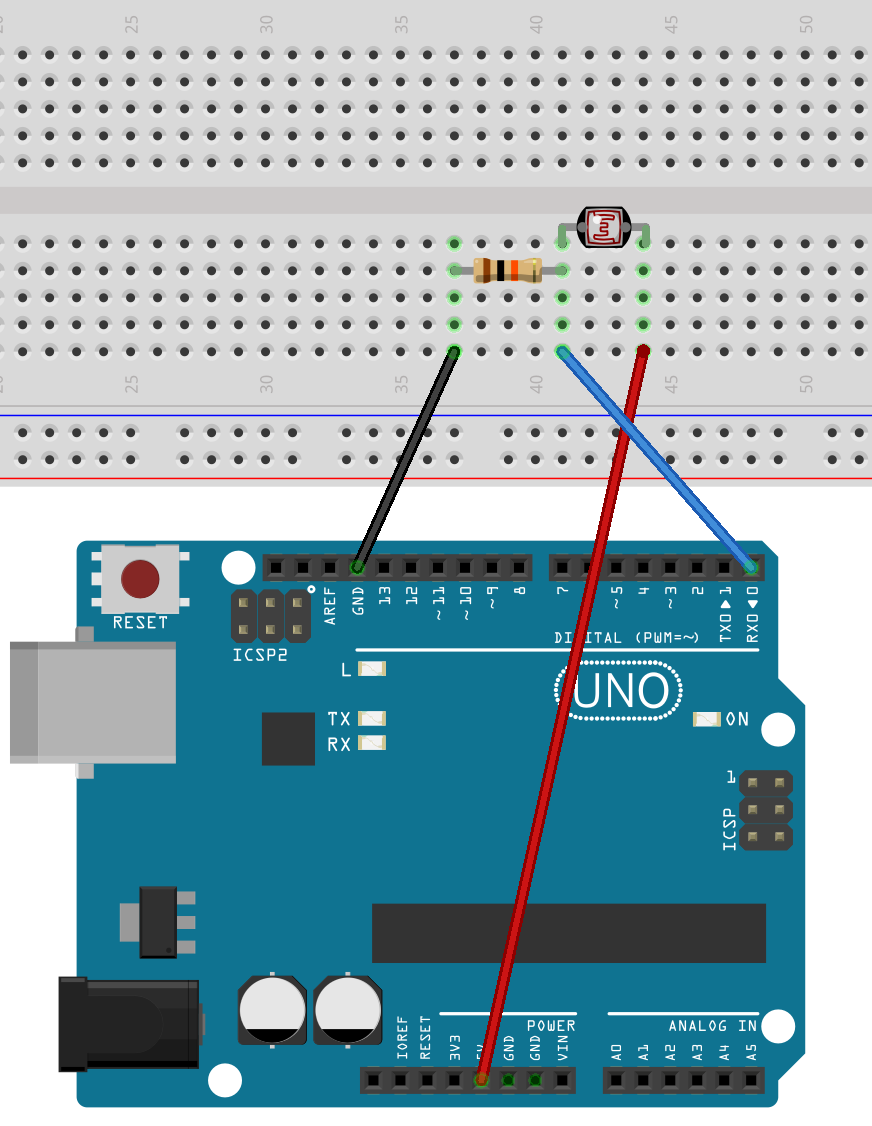
\includegraphics[width=\textwidth]{res/img/resistor}    
            \end{subfigure}
        \caption{Schema över sändare/mottagare}\label{fig:schem}
        \end{figure}


    % subsection optisk_kommunikation (end)
    
% section resultat (end)